\begin{frame}[c]{Nonlinear Schwarz implementation}
\centering
    \begin{tikzpicture}[node distance=2cm]
        \node (start) [startstop] {Init.};
        \node (dec) [decision, right of=start] {Converged?};
        
        \node (evalCalF) [process, right of=dec, xshift=0.5cm] {Evaluate $\mathcal{F}(u^k)$};
        \node (evalDCalF) [process, right of=evalCalF, xshift=0.5cm] {Evaluate $D\mathcal{F}(u^k)$};
        \node (update) [process, above of=evalDCalF, yshift=-0.5cm] {Update $u^k$};
        \node (evalF) [process, above of=evalCalF, yshift=-0.5cm] {Evaluate $F(u^{k+1})$};
        
        \node (stop) [startstop, below of=dec] {Stop};
        
        \draw [arrow] (start) -- (dec);
        \draw [arrow] (dec) -- node[anchor=east] {yes} (stop);
        \draw [arrow] (dec) -- node[anchor=south] {no} (evalCalF);
        \draw [arrow] (evalCalF) -- (evalDCalF);
        \draw [arrow] (evalDCalF) -- (update);
        \draw [arrow] (update) -- (evalF);
        \draw [arrow] (evalF) -| (dec);
    \end{tikzpicture}
\end{frame}

\begin{frame}[c]{Nonlinear Schwarz implementation}
\centering
\def\opacity{0.25}
    \begin{tikzpicture}[node distance=2cm]
        \node (start) [startstop, opacity=\opacity] {Init.};
        \node (dec) [decision, right of=start, opacity=\opacity] {Converged?};
        
        \node (evalCalF) [process, right of=dec, xshift=0.5cm] {Evaluate $\mathcal{F}(u^k)$};
        \node (evalDCalF) [process, right of=evalCalF, xshift=0.5cm, opacity=\opacity] {Evaluate $D\mathcal{F}(u^k)$};
        \node (update) [process, above of=evalDCalF, yshift=-0.5cm, opacity=\opacity] {Update $u^k$};
        \node (evalF) [process, above of=evalCalF, yshift=-0.5cm, opacity=\opacity] {Evaluate $F(u^{k+1})$};
        
        \node (stop) [startstop, below of=dec, opacity=\opacity] {Stop};
        
        \draw [arrow, opacity=\opacity] (start) -- (dec);
        \draw [arrow, opacity=\opacity] (dec) -- node[anchor=east] {yes} (stop);
        \draw [arrow, opacity=\opacity] (dec) -- node[anchor=south] {no} (evalCalF);
        \draw [arrow, opacity=\opacity] (evalCalF) -- (evalDCalF);
        \draw [arrow, opacity=\opacity] (evalDCalF) -- (update);
        \draw [arrow, opacity=\opacity] (update) -- (evalF);
        \draw [arrow, opacity=\opacity] (evalF) -| (dec);
    \end{tikzpicture}
\end{frame}

\begin{frame}{Nonlinear Schwarz: the residual $\mathcal{F}(u^k)$}
    Recall:
    \begin{equation*}
        \mathcal{F}(u) \coloneqq \sum_{i=0}^NP_iT_i(u)
    \end{equation*}
    with $T_i$ defined by 
    \begin{equation*}
        R_iF(u-P_iT_i(u)) = 0, \quad i = 0,1,\dots N
    \end{equation*}
    Requirements for evaluation $\mathcal{F}(u)$
    \begin{enumerate}
        \item Overlapping partition of the mesh
        \item Build coarse basis functions
        \item Solution of $R_iF(u-P_ig_i) = 0$ with $g_i\coloneqq T_i(u)$
        \item Recombination of the local solutions
    \end{enumerate}
\end{frame}



\begin{frame}{Nonlinear Schwarz: the residual $\mathcal{F}(u^k)$}
    \begin{columns}
        \begin{column}{0.5\textwidth}
            \vfill
            \hspace*{10pt}
            Nonlinear corrections 
            \hspace*{20pt}
            \begin{align*}
                \hspace*{6pt}-\nabla\cdot((u^2+1)\nabla u)&=10\quad \text{in}\quad \Omega\subset\mathbb{R}^2,\\
                        u &= 0\quad\text{on}\quad\partial\Omega
            \end{align*}
            \hspace*{10pt}with $u^0 = 1$
        \end{column}
        \begin{column}{0.5\textwidth}
            \begin{figure}
                \centering
                \scalebox{1}{\begin{tikzpicture}
\node[inner sep=0pt] (peak) at (0,0)
    {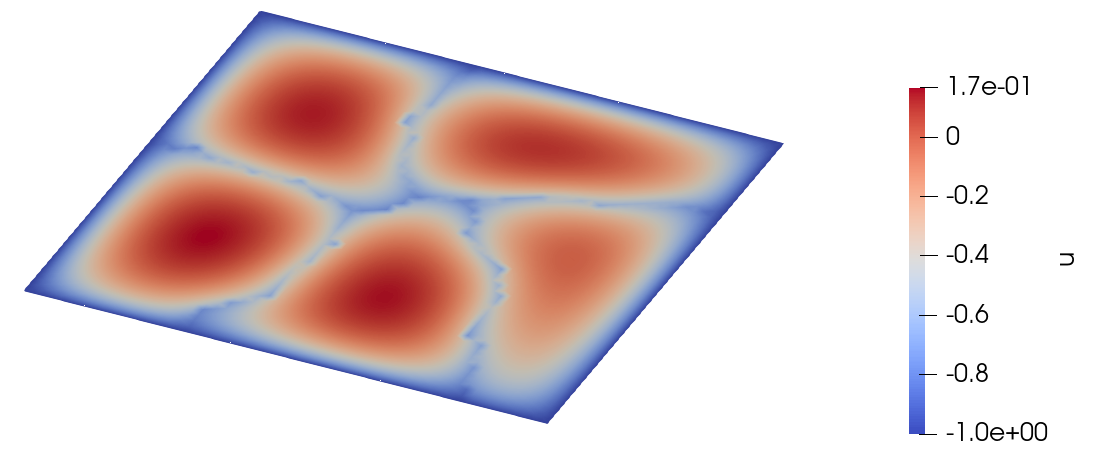
\includegraphics[width=0.9\textwidth]{images/base1.png}};
\node[inner sep=0pt] (peak1) at (1.5,-3.8)
    {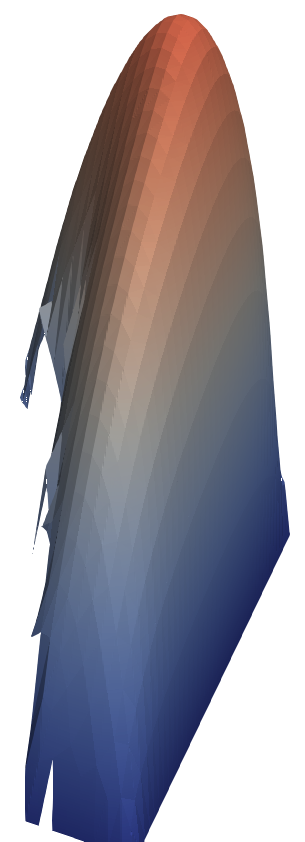
\includegraphics[width=.15\textwidth,height=0.3\textwidth]{images/peak1.png}};
\draw[->,thick] (0.2,-0.6) -- (peak1.north) node[midway,fill=white] {\footnotesize $T_1(u^0)$};
\node[inner sep=0pt] (peak2) at (-2.5,-3.8)
    {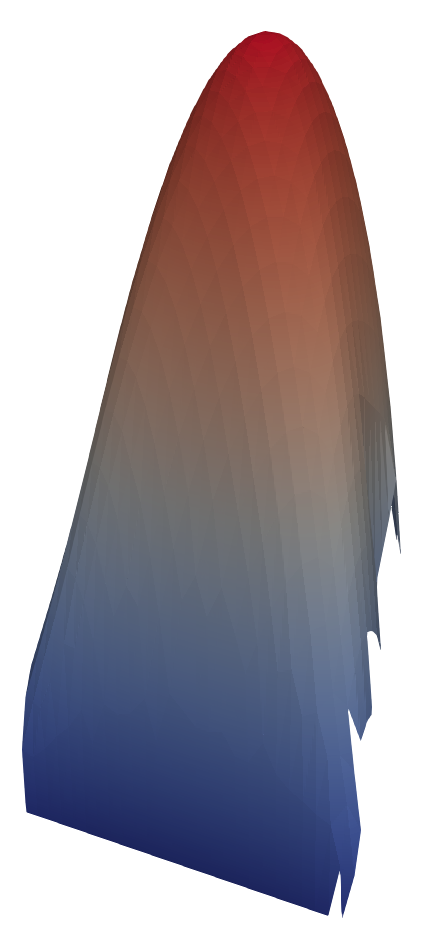
\includegraphics[width=.2\textwidth,height=0.34\textwidth]{images/peak2.png}};
\draw[->,thick] (-1.4,-0.6) -- (-2.2,-2.3)node[midway,fill=white] {\footnotesize $T_2(u^0)$};
\end{tikzpicture}}
            \end{figure}   
        \end{column}
    \end{columns}
    
    
\end{frame}

\begin{frame}[c]{Nonlinear Schwarz implementation}
    \centering
    \def\opacity{0.25}
    \begin{tikzpicture}[node distance=2cm]
        \node (start) [startstop, opacity=\opacity] {Init.};
        \node (dec) [decision, right of=start, opacity=\opacity] {Converged?};
        
        \node (evalCalF) [process, right of=dec, xshift=0.5cm, opacity=\opacity] {Evaluate $\mathcal{F}(u^k)$};
        \node (evalDCalF) [process, right of=evalCalF, xshift=0.5cm] {Evaluate $D\mathcal{F}(u^k)$};
        \node (update) [process, above of=evalDCalF, yshift=-0.5cm, opacity=\opacity] {Update $u^k$};
        \node (evalF) [process, above of=evalCalF, yshift=-0.5cm, opacity=\opacity] {Evaluate $F(u^{k+1})$};
        
        \node (stop) [startstop, below of=dec, opacity=\opacity] {Stop};
        
        \draw [arrow, opacity=\opacity] (start) -- (dec);
        \draw [arrow, opacity=\opacity] (dec) -- node[anchor=east] {yes} (stop);
        \draw [arrow, opacity=\opacity] (dec) -- node[anchor=south] {no} (evalCalF);
        \draw [arrow, opacity=\opacity] (evalCalF) -- (evalDCalF);
        \draw [arrow, opacity=\opacity] (evalDCalF) -- (update);
        \draw [arrow, opacity=\opacity] (update) -- (evalF);
        \draw [arrow, opacity=\opacity] (evalF) -| (dec);
    \end{tikzpicture}
\end{frame}

\begin{frame}{Nonlinear Schwarz: the tangent $D\mathcal{F}(u^k)$}
    Recall: 
    \begin{equation*}
        D\mathcal{F}(u^k) =\sum_{i=0}^NP_i(R_iDF(u_i^k)P_i)^{-1}R_iDF(u_i^k)
    \end{equation*}
    with $u_i = u-P_iT_i(u)$\\~\\
    \begin{itemize}
       \setlength{\itemsep}{10pt}
        \item Requires assembly of Jacobian $DF(u_i^k)$ on each subdomain
        \item This is already done in local and coarse Newton methods \\$\implies$ stored and reused to assemble $D\mathcal{F}(u^k)$
    \end{itemize}
\end{frame}


\begin{frame}{Software ecosystem}
    \begin{tikzpicture}[node distance = 1cm, auto]

	\node [whtblock,text depth=14mm] (FEDDLIB) {
		{\footnotesize \textbf{FEDDLib}\textsuperscript{a}} \\[0.3em] \tiny \textbf{F}inite \textbf{E}lement and \textbf{D}omain \textbf{D}ecomposition \textbf{Lib}rary
		\begin{itemize}
			\item{Parallel finite element assembly}
			\item{Specific problem definition}
			\item{Mesh handling routines}
			      % \item \textcolor{orange}{Update two-level nonlinear Schwarz solver for elasticity and Navier-Stokes}
			      % \item \textcolor{orange}{Test with various coarse spaces}
		\end{itemize}
		% \hspace*{-25mm}\scalebox{.7}{By University of Cologne, TU Delft, TU Freiberg}
	};

	\node [whtblock, right=of FEDDLIB,node distance=7cm, rectangle split part fill={orange!20,blue!5},] (FeatFlow) {
		{ \footnotesize\textbf{FEAT3}\textsuperscript{b}}\\[0.3em] \tiny Finite element based solution of incompressible\\Navier-Stokes in 2D and 3D
		\vspace{2pt}
		\begin{itemize}
			%\setlength{\itemsep}{0pt}
			\item \textcolor{red}{Interface with \texttt{FROSch}}
			\item \textcolor{red}{Test (non-Newtonian, high Reynolds, exascale)}
		\end{itemize}};

	%===============================================    
	\node [whtblock, below=of FEDDLIB, text depth=18mm, node distance=3.5cm,] (Trilinos) {
		{\footnotesize \textbf{Trilinos}\textsuperscript{c}}
		\begingroup
		\addtolength{\leftmargini}{0.5cm}
		\vspace{1pt}
		\tiny
		\begin{itemize}
			%\setlength{\itemsep}{0pt}
			\item Data services: Vectors, matrices, graphs and related operations
			\item Linear and Eigenproblem solvers
			\item Nonlinear solvers and analysis tools
		\end{itemize}
		\endgroup
	};

	\node[inner sep=0pt] (trilinos_logo) at ([xshift=6mm, yshift=0mm] Trilinos.west){
\includegraphics[width=.125\textwidth, angle=90,origin=c]{images/logo/Trilinos_logo_new.png}};

	\node [whtblock, text depth=18mm, right=of Trilinos,node distance=7cm,rectangle split part fill={orange!20,blue!5},] (Frosch) {
		{\footnotesize \textbf{FROSch}\textsuperscript{d}} \\[0.4em]  \hspace{6em}\tiny\textbf{F}ast and \textbf{R}obust \textbf{O}verlapping \textbf{S}chwarz
		\vspace*{0.5em}
		\begingroup
		\addtolength{\leftmargini}{4em}
		\begin{itemize}
			\item \textcolor{red}{Implement two-level nonlinear Schwarz solver}
			\item \textcolor{red}{Test with various coarse spaces on various model problems}
		\end{itemize}
		\endgroup
	};

	\node[inner sep=0pt] (trilinos_logo) at ([xshift=7.5mm, yshift=0mm] Frosch.west){
\includegraphics[width=.1\textwidth]{images/logo/FROSch_logo.png}};

	%%%%%%%%%%%%%%%%%%%%%%%%%%%%%%%%
	%   CONTAINERS -- BACKGROUND LIGHT-DASHED BLOCKS
	%%%%%%%%%%%%%%%%%%%%%%%%%%%%%%%%
	\begin{scope}[on background layer]

		\coordinate (aux2) at ([yshift=0mm]Trilinos.north);
		\node[container2, fit=(aux2) (Trilinos) (Frosch)] (Trilinos_blue) {};

		\coordinate (aux3) at ([yshift=0mm] FeatFlow.north);
		\node[container3, fit=(aux3) (FeatFlow)] (FeatFlow_Green) {};

		\coordinate (aux1) at ([yshift=0mm]FEDDLIB.north);
		\node [container,fit=(aux1) (FEDDLIB)] (FEDDLIB_ORANGE) {};
		\node at ([yshift=0.7mm]Trilinos_blue.north) [fill=gray!10,draw,minimum width=8em,minimum height=1em] (FEDTRI-label) {\footnotesize\textbf{Interface}};

	\end{scope}
	%************************************************************
	%************************************************************
	%  Draw edges
	%************************************************************
	%************************************************************
	% \path [line,thick] (FEDDLIB) -- (FEDTRI-label);
	% \path [line,thick] (Trilinos) -- (Frosch);
	% \path [line,thick] (FEDTRI-label) -- (Trilinos);
	% \path [line,red,thick] (FeatFlow) -- (FEDTRI-label);

\end{tikzpicture}
\tiny\\~\\

a: University of Cologne, TU Delft, TU Freiberg (https://github.com/FEDDLib/FEDDLib.git)\\
b: TU Dortmund (https://github.com/tudo-math-ls3/feat3)\\
c: Sandia National Laboratories (https://trilinos.github.io)\\
d: University of Cologne, TU Delft, TU Freiberg (https://shylu-frosch.github.io)\\

\end{frame}